\chapter{线性代数}
\label{ch:linear_algebra}

线性代数是广泛使用在整个科学和工程中的一个数学分支。然而,由于线性代数是一种连续
的形式而不是离散数学,许多计算机科学家对它少有经验。很好地理解线性代数,对理解和
使用许多\gls*{ml}算法来工作,是必不可少的,对\gls*{dl}尤其如此。因此,我们在介
绍\gls*{dl}之前先专注于对关键的线性代数必备知识做些陈述。

如果你已经熟悉了线性代数,尽管跳过这一章。如果你对这些概念有了一些先期的经验,但
是需要一个详细的参考来复习关键的公式,我们推荐 \emph{The Matrix Cookbook}
\citep{matrix-cookbook}。如果你完全没有接触过线性代数,这一章会教你足够的知识来阅
读本书,但是我们强烈建议你也去咨询其它专门教授线性代数的材料,例
如\citep{shilov1977linear}。本章会完全略过很多重要的线性代数的主题,它们对理
解\gls*{dl}不是必须的。

\section{标量、向量、矩阵和张量}
\label{scalars_vectors_matrices_and_tensors}

线性代数的研究涉及到几种数学对象的类型:

\begin{itemize}
\item \emph{\gls{scalars}}:一个\gls*{scalar}仅仅是一个单独的数字,相反,大多数其
  它线性代数的研究对象通常是多个数组。我们用斜体来写\gls*{scalar}。我们通常用小写
  命名\gls*{scalar}。当我们介绍它们时,我们指定它们是什么样的数字。例如:当定义一
  个实数值的\gls*{scalar}时,我们可能说``设 $s \in \mathbb{R}$ 为直线的斜率'',或
  者,当定义一个自然数\gls*{scalar}时,``设 $n \in \mathbb{N}$ 为单元的个数''。
\item \emph{\gls{vectors}}:一个\gls*{vector}是一个数组。这些数字按照顺序排列。我
  们可以通过这一顺序中的索引来确定每一个单独的数字。通常我们以小写的粗体字体
  给\gls*{vector}命名,例如 $\pmb{x}$。\gls*{vector}的元素以伴有下标的斜体字体表
  示。$\pmb{x}$
  的第一个元素是$x_1$,第二个是$x_2$,依此类推。我们还要说明\gls*{vector}中存储的
  是什么类型的数字。如果每个元素是 $\mathbb{R}$ 中的数,而\gls*{vector}有 $n$ 个
  元素,那么\gls*{vector}位于以 $\mathbb{R}$ 的 $n$ 次笛卡尔积的所形成的集合内,
  表示为$\mathbb{R}^n$。当我们需要显式地表示一个\gls*{vector}中的元素,我们把它们
  写成方括号围起来的一列:
  \begin{equation}
    x = \begin{bmatrix}x_1\\ x_2\\ \vdots\\ x_n\end{bmatrix}
    \label{eq:vector_example}
  \end{equation}
  我们可以把\gls*{vector}看做表示空间的点,每个元素提供沿着不同坐标轴的坐标。\\
  有时候我们需要索引一个向量中的一个元素集合。在这种情况下,我们定义一个包含索引
  的集合,并把这个集合写成一个下标。例如,为了获得 $x_1$,$x_3$ 和 $x_6$,我们定
  义集合 $S = {1, 3, 6}$,写为 $\pmb{x}_S$。我们使用 $-$ 标记表示一个集合的补充。
  例如 $\pmb{x}_{-1}$ 是包含 $\pmb{x}$ 中除了 $x_1$ 的所有元素
  的\gls*{vector},而 $\pmb{x}_{-S}$ 是包含 $\pmb{x}$ 中除
  了 $x_1$,$x_2$ 和 $x_6$ 之外的所有元素的向量。
\item \emph{\gls{matrices}}:一个矩阵是一个数字的二维数组,所以每个元素由两个索引
  确定,而不是一个。我们通常用大写的粗体字体表示矩阵,例如 $\pmb{A}$。如果一个实
  数值的矩阵 $\pmb{A}$ 高度为 $m$,宽度为 $n$,那么我们说
  $\pmb{A} \in \mathbb{R}^{m \times n}$。我们通常使用斜体~——~但不是粗体字体~——~表
  示一个矩阵的元素,索引用逗号分开列出。例如,$A_{1,1}$ 是 $\pmb{A}$ 左上角的元素,
  而 $A_{m,n}$ 是右下角的元素。我们可以为横向坐标写一个 ``:'' 来表示所有竖向坐
  标 $i$ 的数字。例如,$\pmb{A}_{i,:}$ 表示竖向坐标 $i$ 的横跨 $\pmb{A}$ 的部分。
  即 $\pmb{A}$ 的第 $i$ 行。同样的,$\pmb{A}_{:,i}$ 是 $\pmb{A}$ 的第 $i$ 列。当
  我们需要显式地表示一个矩阵的元素,我们把它们写成一个用方括号围起来的数组:
  \begin{equation}
    \begin{bmatrix}A_{1,1} & A_{1,2} \\ A_{2,1} & A_{2,2}\end{bmatrix}
    \label{eq:matrix_example}
  \end{equation}
  有时候我们可能需要索引矩阵值的表达式,它不仅仅是一个单个的字母。在这种情况下,
  我们在表达式后使用下标,但不转换为小写。例如,$f(\pmb{A})_{i,j}$ 给出了应用函
  数 $f$ 到 $\pmb{A}$ 上后计算得到的 $(i,j)$ 位置的元素。。
\item \emph{\gls{tensors}}:在有些情况下我们会需要一个多于两个坐标的数组。在一般
  情况下,排列在一个规则的网格~——~具有可变数量的坐标轴~——~上的数组,被称为一
  个\emph{\gls{tensor}}。我们用这样的字体表示一个名为 ``A'' 的张
  量:$\pmb{\mathsf{A}}$。我们把表示 $\pmb{\mathsf{A}}$ 在 $(i,j,k)$ 坐标的元素写
  为 $\mathsfit{A}_{i,j,k}$。
\end{itemize}

矩阵的一个重要的操作是\emph{\gls{transpose}}。一个矩阵的\gls*{transpose}是将矩阵
沿着一个对角线~——~称为\emph{\gls{main-diag}},从左上角指向右下角~——~做镜像。参见
图~\ref{fig:transpose_of_matrix} 中对这个操作的图形化描述。我们把一个矩
阵 $\pmb{A}$ 的转置表示为 $\pmb{A}^{\top}$,以这样定义
\begin{equation}
  (\pmb{A}^{\top})_{i,j} = A_{j,i}
  \label{eq:transpose_of_matrix}
\end{equation}

\begin{figure}[h]
  \centering
  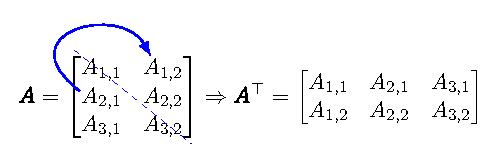
\includegraphics{transpose_of_matrix}
  \caption{矩阵的转置可以被看做沿着\gls*{main-diag}的镜
    像\label{fig:transpose_of_matrix}}
\end{figure}

\gls*{vectors}可以被看做是只含有一列的\gls*{matrix}。如此一
个\gls*{vector}的\gls*{transpose}就是一个只有一行的\gls*{matrix}。有时候这样定义
一个\gls*{vector}:在一行的\gls*{matrix}的文本区中写出它的元素,然后使用一
个\gls*{transpose}操作来把它转换成标准的列\gls*{vector},例如,$\pmb{x} = [x_1,
x_2, x_3]^{\top}$。

一个\gls*{scalar}可以被看做是只有一个元素的\gls*{matrix}。因此,我们可以看到一
个\gls*{scalar}就是它自己的\gls*{transpose}:$a = a^{\top}$。

只要\gls*{matrices}有相同的形状,我们可以把它们相互相加,只需要将它们对应的元素相
加:$\pmb{C} = \pmb{A} + \pmb{B}$,这里 $C_{i,j} = A_{i,j} + B_{i,j}$。

我们也可以把一个\gls*{scalar}加到一个\gls*{matrix}上,或者用一个\gls*{scalar}乘以
一个\gls*{matrix},只需要在\gls*{matrix}上执行操作:$\pmb{D} = a \cdot \pmb{B} +
c$,这里 $D_{i,j} = a \cdot B_{i,j} + c$。

在\gls*{dl}的环境中,我们也使用一些较传统的符号。我们允许\gls*{matrix}和一
个\gls*{vector}相加,产生另一个\gls*{matrix}:$\pmb{C} = \pmb{A} + \pmb{b}$,这
里 $C_{i,j} = A_{i,j} + b_j$。换句话说,\gls*{vector} $\pmb{b}$ 被加
到\gls*{matrix}的每一行。这个速记法消除了需要在相加前定义一个复制 $\pmb{b}$ 到每
一行的\gls*{matrix}。这个 $\pmb{b}$ 到多个位置的隐式拷贝被称
为\emph{\gls{broadcasting}}。

\section{矩阵和向量的乘法}
\label{sec:multiplying_matrices_and_vectors}

涉及\gls*{matrices}的最重要的操作之一是两个\gls*{matrix}的乘法。\gls*{matrices}
$\pmb{A}$ 和 $\pmb{B}$ 的\emph{\gls{matrix-product}}\,是另一个\gls*{matrix}
$\pmb{C}$。为了这种积可定义,$\pmb{A}$ 的列数量必须和 $\pmb{B}$ 的行数相同。如
果 $\pmb{A}$ 的形状为 $m \times n$,而 $\pmb{B}$ 的形状为 $n \times p$,那
么 $\pmb{C}$
的形状为$m \times p$。我们可以把两个或更多\gls*{matrices}放在一起来
写\gls*{matrix-product},例如:
\begin{equation}
  \pmb{C} = \pmb{A}\pmb{B}
  \label{eq:matrix_product}
\end{equation}

乘积操作被定义为:
\begin{equation}
  C_{i,j} = \sum_{k}A_{i,k}B_{k,j}
  \label{eq:product_operation}
\end{equation}

注意两个\gls*{matrices}的标准乘积\textbf{不}仅仅是一个包含有单独元素乘积
的\gls*{matrix}。这样的操作是存在的,并被称
为\emph{\gls{element-product}}\,或者\emph{\gls{hadamard-product}},表示
为 $\pmb{A} \odot \pmb{B}$。

两个具有相同维度的\gls*{vectors}
$\pmb{x}$ 和 $\pmb{y}$ 的\emph{\gls{dot-product}}\,是\gls*{matrix-product}
$\pmb{x}^{\top}\pmb{y}$。我们可以把\gls*{matrix-product} $\pmb{C} =
\pmb{A}\pmb{B}$ 看做计
算 $\pmb{A}$ 的第 $i$ 行和 $\pmb{B}$ 的第 $j$ 列的\gls*{dot-product} $C_{i,j}$。

\gls*{matrix-product}操作有很多有用的特性,使得对\gls*{matrices}的数学分析更方
便。例如,\gls*{matrix}的乘法是可分配的:
\begin{equation}
  \pmb{A}(\pmb{B} + \pmb{C}) = \pmb{A}\pmb{B} + \pmb{A}\pmb{C}
  \label{eq:distributive_matrix_multiplication}
\end{equation}
也可结合:
\begin{equation}
  \pmb{A}(\pmb{B}\pmb{C}) = (\pmb{A}\pmb{B})\pmb{C}
  \label{eq:associative_matrix_multiplication}
\end{equation}
不像\gls*{scalar}乘法,\gls*{matrix}乘法是\textbf{不}可交换的($\pmb{A}\pmb{B} =
\pmb{B}\pmb{A}$ 的条件并不总是成立)。但是,两个\gls*{vectors}之间
的\gls*{dot-product}是可交换的:
\begin{equation}
  \pmb{x}^{\top}\pmb{y} = \pmb{y}^{\top}\pmb{x}
  \label{eq:commutative_vector_multiplication}
\end{equation}

\gls*{matrix-product}的\gls*{transpose}有一个简单的形式:
\begin{equation}
  (\pmb{A}\pmb{B})^{\top} = \pmb{B}^{\top}\pmb{A}^{\top}
  \label{eq:transpose_of_matrix_product}
\end{equation}

这使我们利用这样一个乘积值为一个标量时,它和自己的\gls*{transpose}相等的事实,来
证明方程~\ref{eq:commutative_vector_multiplication}:
\begin{equation}
  \pmb{x}^{\top}\pmb{y} = (\pmb{x}^{\top}\pmb{y})^{\top} = \pmb{y}^{\top}\pmb{x}
  \label{eq:demonstrate_commutative_vector_multiplication}
\end{equation}

由于这本教科书的重点不是线性代数,我们在这里不会试图列出全面
的\gls*{matrix-product}的有用特性,但读者应该知道有更多。

现在我们知道了足够的线性代数的数学符号来写下一个线性方程的系统:
\begin{equation}
  \pmb{A}\pmb{x} = \pmb{b}
  \label{eq:system_of_linear_equations}
\end{equation}
这里 $\pmb{A} \in \mathbb{R}^{m \times
  n}$是一个已知的\gls*{matrix},$\pmb{b} \in \mathbb{R}^m$ 是一个已知
的\gls*{vector},而 $\pmb{x} \in \mathbb{R}^n$ 是一个我们想要解出的未知变量
的\gls*{vector}。$\pmb{A}$ 的每一行和 $\pmb{b}$ 的每个元素提供了另一个限制。我们
可以重写方程~\ref{eq:system_of_linear_equations} 为:
\begin{align}
  \pmb{A}_{1,:}\pmb{x} &= b_1\\
  \pmb{A}_{2,:}\pmb{x} &= b_2\\
  \ldots \\
  \pmb{A}_{m,:}\pmb{x} &= b_m
\end{align}

或者,甚至更明确地:
\begin{align}
  \pmb{A}_{1,1}x_1 + \pmb{A}_{1,2}x_2 + \ldots + \pmb{A}_{1,n}x_n = b_1 \\
  \pmb{A}_{2,1}x_1 + \pmb{A}_{2,2}x_2 + \ldots + \pmb{A}_{2,n}x_n = b_2 \\
  \ldots & \\
  \pmb{A}_{m,1}x_1 + \pmb{A}_{m,2}x_2 + \ldots + \pmb{A}_{m,n}x_n = b_m
\end{align}

\gls*{matrix}--\gls*{vector}乘积的符号提供了这种方程形式的一个更紧凑的表示。

\section{单位矩阵和逆矩阵}
\label{sec:identity_and_inverse_matrices}

线性代数提供一个强大的工具,被称为\emph{\gls{matrix-inversion}},允许我们以分析
的方法解不同值的 $\pmb{A}$ 的方程~\ref{eq:system_of_linear_equations}。

为了描述\gls*{matrix-inversion},我们首先需要定义一个
\emph{\gls{identity-matrix}}\,的概念。一个\gls*{identity-matrix}是这样一个矩阵,
把它乘以任何\gls*{vector}都不会改变\gls*{vector}。我们将保留 $n$ 维
\gls*{vectors}的\gls*{identity-matrix}表示为 $\pmb{I}_n$。正式地,$\pmb{I}_n \in \mathbb{R}^{n \times n}$,并且
\begin{equation}
  \forall \pmb{x} \in \mathbb{R}^n, \pmb{I}_n\pmb{x} = \pmb{x}
  \label{eq:definition_of_identity_matrix}
\end{equation}

\gls*{identity-matrix}的结构很简单:所有沿着主对角线的元素是 $1$,同时其它元素是
$0$。参见图~\ref{fig:identity_matrix} 的示例。

\begin{figure}[h]
  \centering
  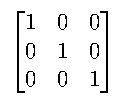
\includegraphics{identity_matrix}
  \caption{\gls*{identity-matrix}的示例:这是
    $\pmb{I}_3$\label{fig:identity_matrix}}
\end{figure}

$\pmb{A}$ 的\gls*{matrix-inversion}表示为 $\pmb{A}^{-1}$,它被定义为这样的矩阵:
\begin{equation}
  \pmb{A}^{-1}\pmb{A} = \pmb{I}_n
  \label{eq:matrix-inverse}
\end{equation}

现在我们可以通过以下步骤解方程~\ref{eq:system_of_linear_equations}:
\begin{align}
  \pmb{A}\pmb{x} &= \pmb{b} \\
  \pmb{A}^{-1}\pmb{A}\pmb{x} &= \pmb{A}^{-1}\pmb{b} \\
  \pmb{I}_n\pmb{x} &= \pmb{A}^{-1}\pmb{b} \\
  \pmb{x} &= \pmb{A}^{-1}\pmb{b}
\end{align}

当然,这依赖于可能找到 $\pmb{A}^{-1}$。我们在接下来一节中讨论 $\pmb{A}^{-1}$ 存
在的条件。

当 $\pmb{A}^{-1}$ 存在时,存在几种不同算法用于在闭合式中找到它。理论上,同样的逆
矩阵可以被用于多次解不同 $\pmb{b}$ 值的方程。然而,$\pmb{A}^{-1}$ 主要作为一个假
设的工具使用,实际上不应该被用在大多数软件应用中。由于在一个数字计算机中
$\pmb{A}^{-1}$ 可以仅由有限精度表示,利用 $\pmb{b}$ 值的算法通常可以取得更精确的
$\pmb{x}$ 的估算。

\section{线性依赖和跨度}
\label{sec:linear_dependence_and_span}
